\section{Resultados e Discussão}
\label{sec:resultados}

\subsection{Dados analisados}

A Tabela~\ref{tab:dados} resume os dados em cada etapa do tratamento. A perda mais
importante ocorre no filtro de cobertura: das 995 viagens com algum registro de GPS, só 431
tinham horário de passagem calculado em pelo menos metade das paradas. A Tabela~\ref{tab:faixas}
mostra que as viagens analisadas se concentram no entrepico de dias úteis; há apenas 7 viagens
de dias úteis com partida entre 16h e 20h, porque a API devolveu poucos registros nesse
período.

\begin{table}[htbp]
\centering
\caption{Volume de dados em cada etapa.}
\label{tab:dados}
\begin{tabular}{lr}
\toprule
Etapa & Quantidade \\
\midrule
Registros brutos de GPS & 105.207 \\
Registros após remover posições repetidas & 41.643 \\
Viagens reais (data + \textit{trip\_id} + veículo) & 995 \\
Viagens com passagem em $\geq$ 50\% das paradas & 431 \\
Viagens na análise (sem duplicatas) & 393 \\
Horários de passagem estimados & 21.871 \\
Trechos usados na réplica (60 trechos) & 21.372 \\
\bottomrule
\end{tabular}
\end{table}

\begin{table}[htbp]
\centering
\caption{Viagens analisadas por tipo de dia e faixa horária da partida programada.}
\label{tab:faixas}
\begin{tabular}{lrrrr}
\toprule
Tipo de dia & Até 9h & 9h--16h & 16h--20h & Após 20h \\
\midrule
Dia útil & 15 & 300 & 7 & 18 \\
Sábado & 2 & 24 & 8 & 8 \\
Domingo & 1 & 5 & 0 & 5 \\
\bottomrule
\end{tabular}
\end{table}

\subsection{Réplica: tempo de deslocamento entre paradas}

A Tabela~\ref{tab:replica} compara o EQM dos modelos com os valores obtidos por
\cite{courb} em Curitiba. A ordem de grandeza e o padrão de melhora são
semelhantes: o maior ganho vem da inclusão do efeito aleatório do trecho (M1 $\rightarrow$
M2), que reduz o EQM em 63\%, e a estrutura AR(1) traz uma redução adicional de 15\%.

\begin{table}[htbp]
\centering
\caption{Erro quadrático médio no ajuste (s$^2$): linha 4110 de Belo Horizonte e linha 863 de
Curitiba \cite{courb}.}
\label{tab:replica}
\begin{tabular}{lrr}
\toprule
Modelo & BH -- linha 4110 & Curitiba -- linha 863 \\
\midrule
M1 -- efeito fixo & 3.688 & 3.420 \\
M2 -- intercepto aleatório por trecho & 1.352 & 969 \\
M3 -- erro AR(1) & 1.150 & 881 \\
M3 sazonal & 1.316 & 851 \\
\bottomrule
\end{tabular}
\end{table}

O intercepto fixo do M2 é de 72,2~s por trecho, com desvio padrão entre trechos de 48,1~s e
desvio padrão residual de 36,8~s. O trecho explica, portanto, 63\% da variância do tempo de
deslocamento (correlação intraclasse). A Figura~\ref{fig:trechos} mostra o tempo previsto para
cada trecho. Os mais lentos estão no início do percurso, entre a Av. Luiz Paulo Franco e a
Av. Raja Gabaglia, passando pela BR-356 (trechos 4 a 6, cada um com cerca de 3,5~minutos), e
na região central, entre a Rua dos Tupis e a Rua Padre Eustáquio (trecho 34, 3,2~minutos). Os
mais rápidos são trechos curtos entre paradas próximas na mesma avenida, com menos de 25~s.

\begin{figure}[htbp]
  \centering
  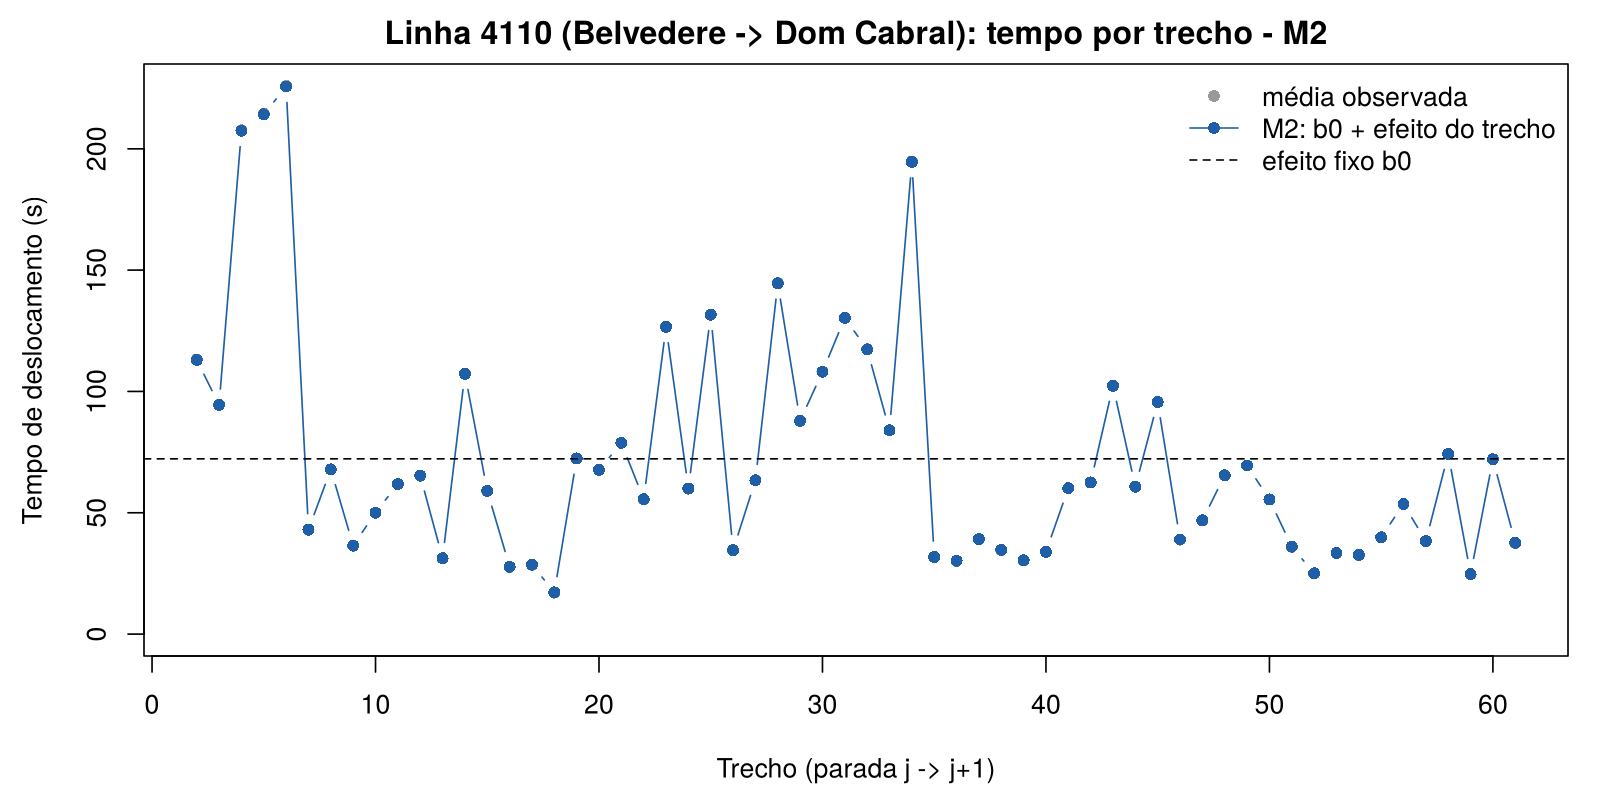
\includegraphics[width=\textwidth]{img/pasquim_efeitos_trecho.png}
  \caption{Tempo de deslocamento médio observado e previsto pelo M2 em cada trecho da linha
  4110 (sentido Belvedere $\rightarrow$ Dom Cabral). A linha tracejada é o efeito fixo
  $\beta_0$.}
  \label{fig:trechos}
\end{figure}

O coeficiente autorregressivo do M3 foi $\phi = 0{,}39$: quando uma viagem é mais lenta que o
esperado em um trecho, a viagem seguinte tende a ser mais lenta no mesmo trecho. A
Figura~\ref{fig:acf} mostra a autocorrelação dos resíduos. No M2 há picos próximos de 60
defasagens, que correspondem ao mesmo trecho na viagem seguinte; esses picos desaparecem no M3
sazonal, cujo componente sazonal estimado foi de 0,43. Ainda assim, o teste de Ljung-Box
indicou autocorrelação residual (p~$<$~0,001), embora pequena em magnitude.

\begin{figure}[htbp]
  \centering
  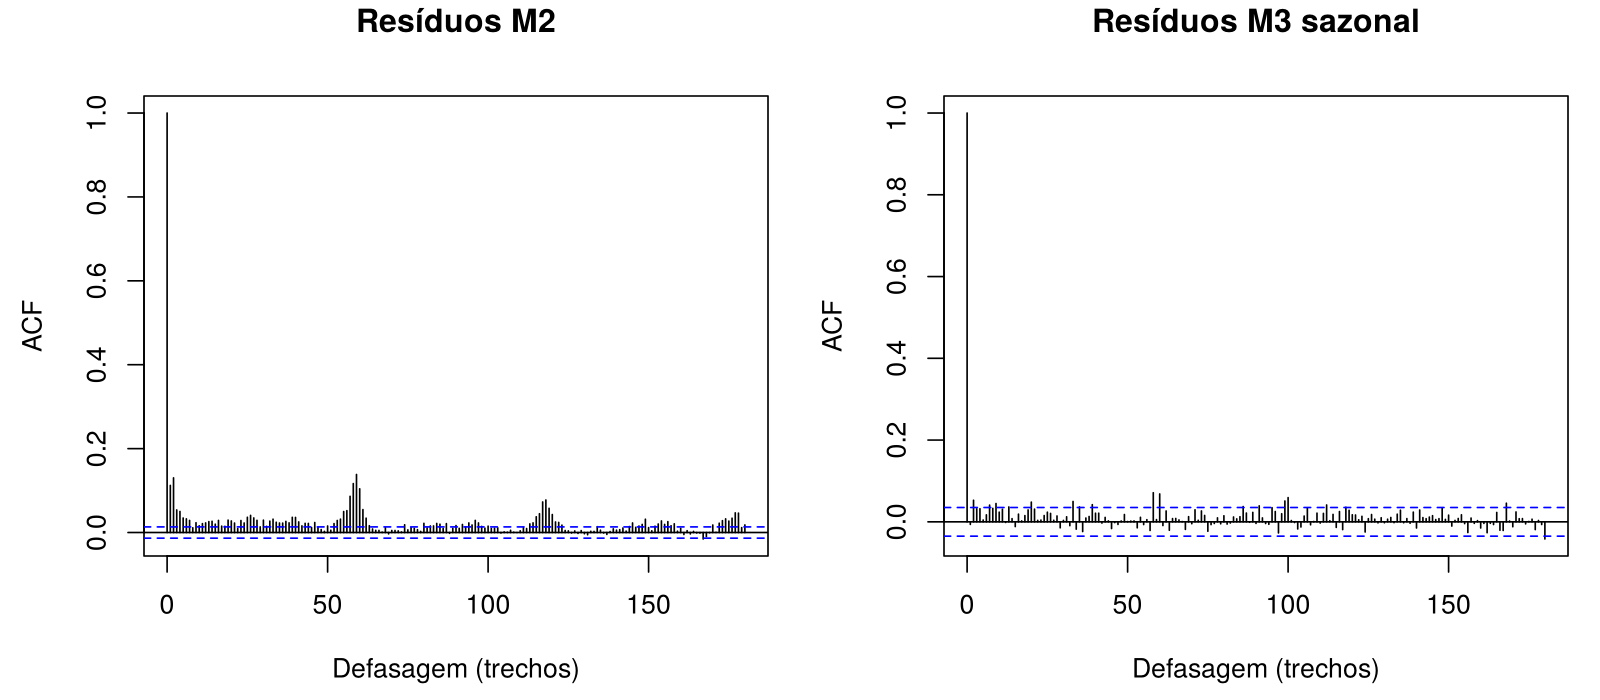
\includegraphics[width=\textwidth]{img/pasquim_acf_residuos.png}
  \caption{Função de autocorrelação dos resíduos do M2 e do M3 sazonal, com defasagem medida
  em trechos.}
  \label{fig:acf}
\end{figure}

Diferentemente de Curitiba, o M3 sazonal não teve o menor EQM. Uma explicação é que, ao
modelar todas as viagens da linha em ordem cronológica, a defasagem sazonal (mesmo trecho,
viagem anterior) coincide com a dependência que o M3 já captura pelo AR(1) dentro do trecho.
No estudo original, com um único veículo, as duas estruturas carregam informações mais
distintas.

A Tabela~\ref{tab:validacao} apresenta a avaliação fora da amostra. Nas duas formas de
validação, o M3 teve o menor RMSE, e o erro típico por trecho caiu de cerca de 60~s no M1 para
cerca de 34~s no M3. O M3 sazonal teve desempenho praticamente igual ao M3. No M2, 95\% das
observações de teste ficaram dentro do intervalo de $\pm 1{,}96\,\sigma$, o que indica que a
variância estimada é adequada. A validação entre quartas-feiras dá resultados próximos aos da
validação com a semana inteira, o que sugere que o padrão por trecho é estável entre as
semanas observadas.

\begin{table}[htbp]
\centering
\caption{Avaliação fora da amostra (erro por trecho, em segundos).}
\label{tab:validacao}
\begin{tabular}{lrrrr}
\toprule
& \multicolumn{2}{c}{Treino 30/03--12/04, teste 13--19/04} & \multicolumn{2}{c}{Treino 08/04, teste 15/04} \\
Modelo & RMSE & MAE & RMSE & MAE \\
\midrule
M1 & 61,8 & 42,7 & 60,0 & 43,1 \\
M2 & 38,6 & 23,0 & 35,5 & 22,3 \\
M3 & 34,8 & 22,1 & 33,7 & 21,6 \\
M3 sazonal & 35,0 & 21,9 & 34,4 & 21,8 \\
\midrule
Observações de teste & \multicolumn{2}{c}{9.556} & \multicolumn{2}{c}{1.787} \\
\bottomrule
\end{tabular}
\end{table}

\subsection{Extensão: atraso em relação ao horário programado}

Nas 258 viagens com registro do início ao fim do percurso, o tempo de viagem observado foi de
69,6~minutos em média (desvio padrão de 7,1), contra 53,1~minutos no quadro de horários. O
atraso médio é de 3,8~minutos na primeira parada com registro e chega a 20,7~minutos na última,
e 85\% dos horários de passagem estão mais de 5~minutos atrasados. A
Figura~\ref{fig:percurso} mostra que o atraso cresce ao longo do percurso, com saltos nos
trechos lentos identificados na réplica: no início (BR-356) e entre os km 7,5 e 11, na
chegada ao centro pela Av. Álvares Cabral e pela Rua São Paulo.

\begin{figure}[htbp]
  \centering
  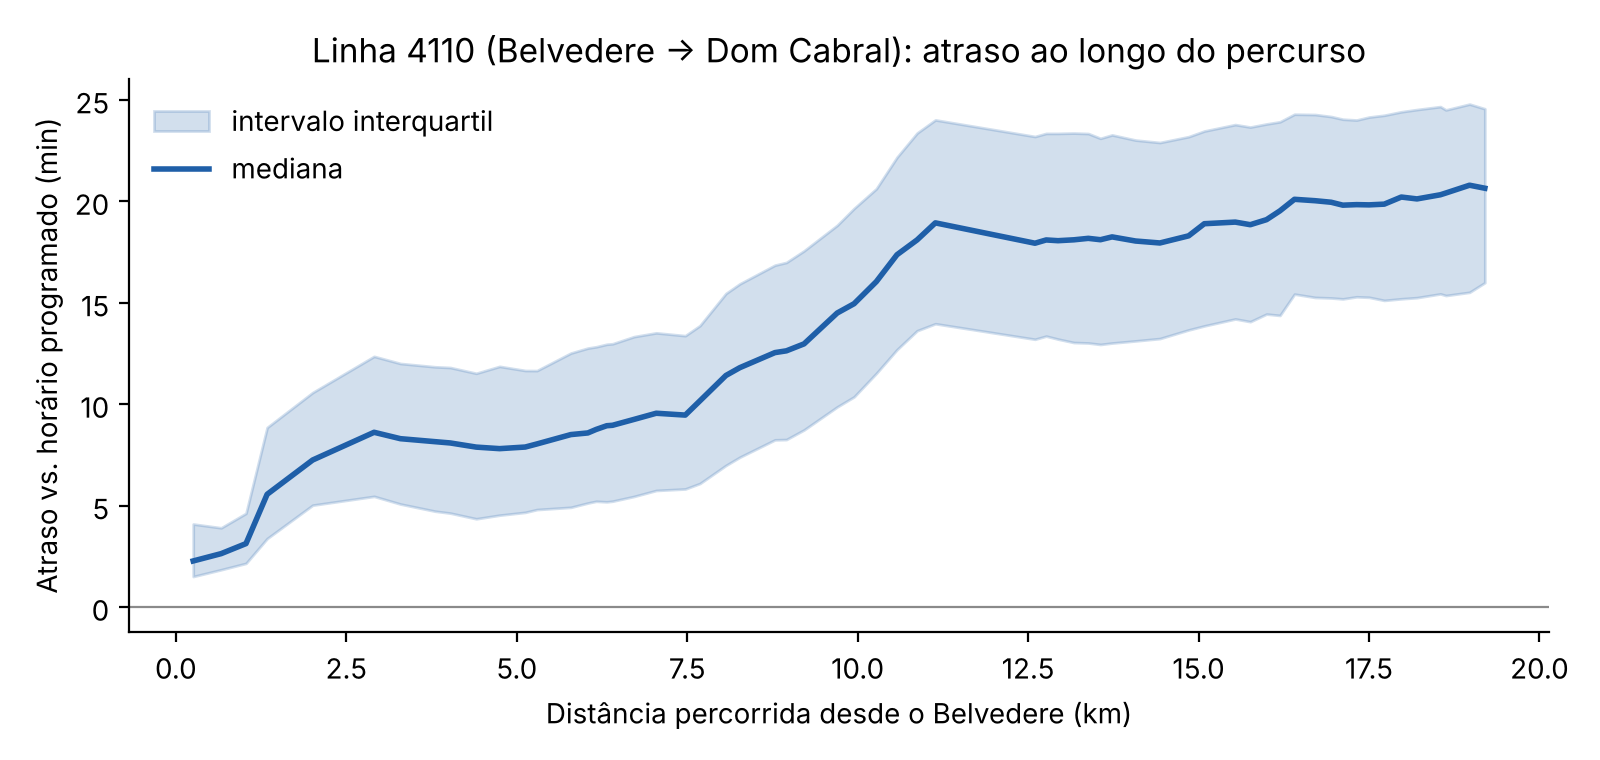
\includegraphics[width=\textwidth]{img/atraso_ao_longo_percurso.png}
  \caption{Atraso em relação ao horário programado ao longo do percurso (mediana e intervalo
  interquartil por parada).}
  \label{fig:percurso}
\end{figure}

A Tabela~\ref{tab:atraso} apresenta os modelos do atraso. No modelo E2, cada quilômetro
percorrido acrescenta 0,92~minuto de atraso (IC95\%: 0,86 a 0,98), controlando a faixa horária
e o tipo de dia. Aos domingos o atraso é 11,3~minutos menor que em dias úteis; aos sábados a
diferença não é significativa. Em relação às partidas até 9h, o atraso é 5,2~minutos menor à
noite, e a diferença no entrepico ($-$2,3~minutos) não é significativa. O efeito aleatório da
viagem (desvio padrão de 5,4~minutos) é bem maior que o da parada (1,3~minuto), uma vez controlada a distância: a maior
parte da diferença entre viagens não é explicada pelas variáveis observadas.

\begin{table}[htbp]
\centering
\caption{Modelos mistos do atraso (minutos). Entre parênteses, intervalo de confiança de 95\%.}
\label{tab:atraso}
\small
\begin{tabular}{lccc}
\toprule
Termo & E1 & E1b & E2 \\
\midrule
Intercepto & 14,2 (13,6; 14,7) & 13,3 (12,0; 14,6) & 7,2 (4,6; 9,8) \\
Pico (16h--20h, dia útil) & 3,1 ($-$1,2; 7,3) & 4,1 ($-$2,9; 11,0) & -- \\
Faixa 9h--16h & -- & -- & $-$2,3 ($-$4,9; 0,2) \\
Faixa 16h--20h & -- & -- & 1,1 ($-$2,7; 4,9) \\
Faixa após 20h & -- & -- & $-$5,2 ($-$8,4; $-$2,1) \\
Sábado & -- & -- & $-$0,7 ($-$2,5; 1,2) \\
Domingo & -- & -- & $-$11,3 ($-$14,6; $-$7,9) \\
Distância (por km) & -- & -- & 0,92 (0,86; 0,98) \\
\midrule
DP efeito aleatório & 5,6 (viagem) & 6,0 (\textit{trip\_id}) & 5,4 (viagem); 1,3 (parada) \\
DP residual & 5,6 & 6,9 & 2,6 \\
\bottomrule
\end{tabular}
\end{table}

O efeito do pico da tarde não foi significativo em nenhum modelo. No E1 a estimativa é de
3,1~minutos, com intervalo que inclui o zero, e no E2 o efeito desaparece quando se controla a
distância. Com o critério de cobertura de 25\%, o número de viagens de pico em dias úteis
passa de 7 para 28 e o efeito no E1 sobe para 4,0~minutos (IC95\%: 1,6 a 6,4), mas no E2
continua não significativo (2,6~minutos; IC95\%: $-$0,4 a 5,7). Como as viagens incompletas
tendem a ser observadas só em parte do percurso, o modelo sem a distância confunde a posição
da parada com o efeito do horário. Esses resultados não permitem afirmar que o pico da tarde
aumenta o atraso na linha 4110; permitem apenas dizer que, se esse efeito existe, os dados
coletados são insuficientes para estimá-lo com precisão.

A comparação entre E1 e E1b mostra por que a primeira etapa deste trabalho havia encontrado
um efeito do pico maior: ao agrupar pelo \textit{trip\_id}, viagens de dias diferentes são
tratadas como se fossem a mesma, o que reduz o número de grupos de 393 para 85 e altera tanto
o intercepto quanto o efeito estimado do pico.

\subsection{Comparação entre semanas}

A Tabela~\ref{tab:semanas} compara o atraso médio por viagem em cada dia da semana nas duas
semanas completas de coleta. As diferenças são pequenas (no máximo 0,8~minuto) e não há
tendência de piora na segunda semana. O padrão se repete nas duas: atrasos de 15 a 17~minutos
de terça a sexta, de 13 a 14~minutos no sábado, cerca de 12~minutos na segunda-feira e de 2 a
3~minutos no domingo. A
Figura~\ref{fig:hora} mostra o atraso médio por hora de partida nos dias úteis: as duas
semanas praticamente coincidem entre 10h e 16h, onde há mais viagens, e se afastam nas horas
com poucas viagens, em que a média é instável.

\begin{table}[htbp]
\centering
\caption{Atraso médio por viagem (minutos) e número de viagens em cada dia da semana.}
\label{tab:semanas}
\begin{tabular}{lrrrrr}
\toprule
& \multicolumn{2}{c}{Semana 1 (06--12/04)} & \multicolumn{2}{c}{Semana 2 (13--19/04)} & \\
Dia & Atraso & Viagens & Atraso & Viagens & Diferença \\
\midrule
Segunda & 11,4 & 35 & 11,9 & 36 & 0,5 \\
Terça & 15,3 & 34 & 15,2 & 24 & $-$0,1 \\
Quarta & 15,8 & 29 & 15,0 & 33 & $-$0,8 \\
Quinta & 16,1 & 15 & 15,6 & 32 & $-$0,5 \\
Sexta & 16,8 & 15 & 16,7 & 28 & $-$0,1 \\
Sábado & 14,1 & 26 & 13,3 & 16 & $-$0,8 \\
Domingo & 2,5 & 5 & 2,3 & 6 & $-$0,2 \\
\bottomrule
\end{tabular}
\end{table}

\begin{figure}[htbp]
  \centering
  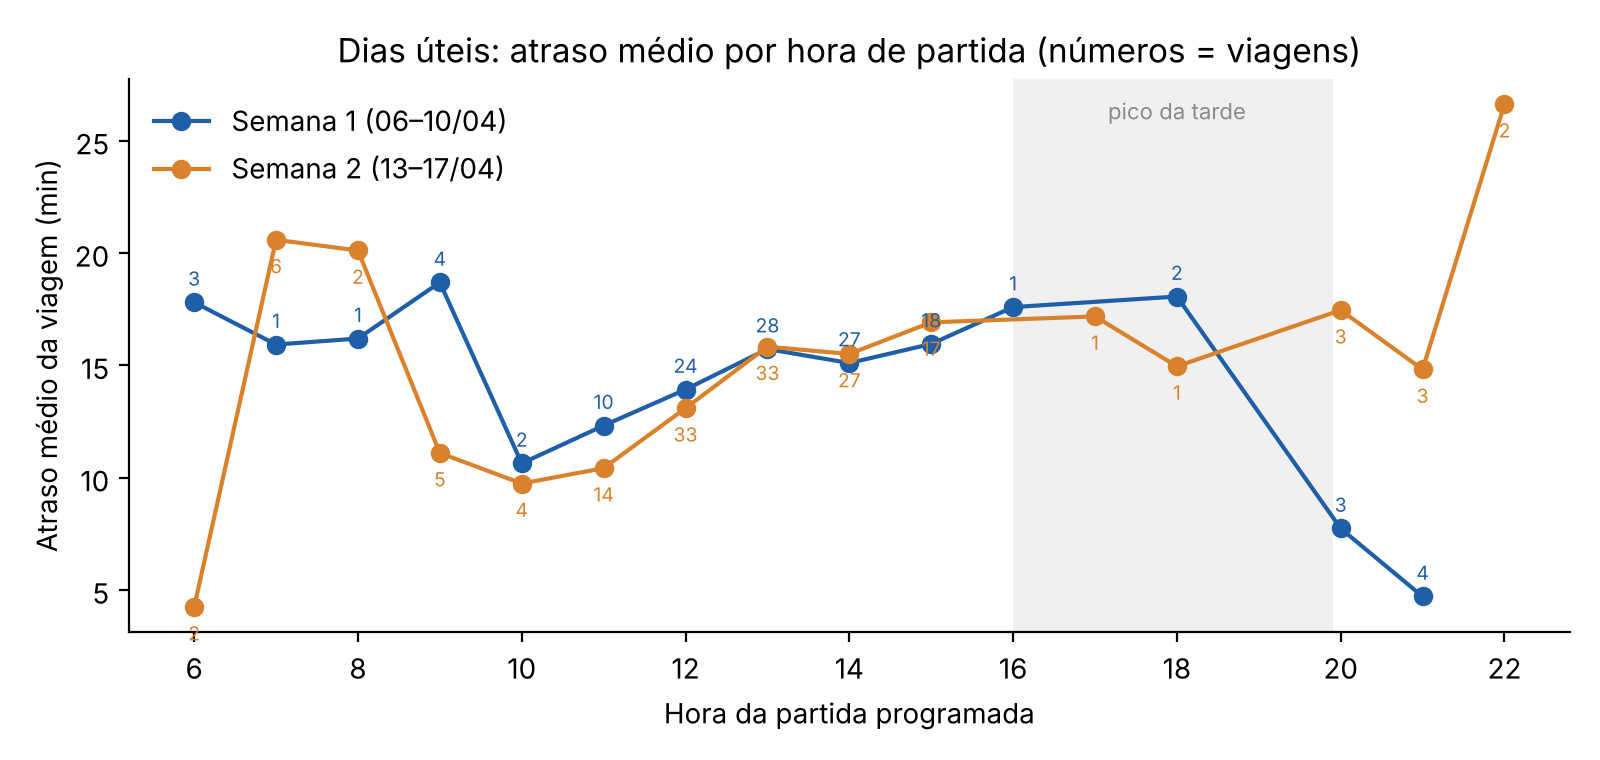
\includegraphics[width=\textwidth]{img/atraso_por_hora_semanas.png}
  \caption{Atraso médio por hora de partida programada em dias úteis, nas duas semanas. Os
  números indicam a quantidade de viagens em cada ponto.}
  \label{fig:hora}
\end{figure}

\subsection{Discussão}

Os resultados reproduzem o principal achado de \cite{courb}: o trecho
é a maior fonte de variabilidade do tempo de deslocamento, e existe dependência entre viagens
sucessivas. Isso indica que a metodologia é transferível entre cidades e fontes de dados, desde
que as diferenças de formato sejam tratadas, como a reutilização dos \textit{trip\_ids} e a
frequência real de atualização do GPS. A estabilidade dos modelos entre semanas reforça que o
padrão por trecho é estrutural.

A extensão mostra que a linha opera, de forma sistemática, com tempo de viagem cerca de 30\%
maior que o programado. O crescimento do atraso ao longo do percurso é compatível com o
acúmulo de atrasos descrito por \cite{Zhang2024} e com a observação
de \cite{doi:10.1177/0361198106195500103} de
que um quadro de horários que não reflete a operação real é, ele mesmo, uma fonte de atraso.
Como os horários intermediários do GTFS são estimativas, parte do atraso medido pode vir dessa
estimativa e não da operação. Ainda assim, a diferença de 16,5~minutos no tempo total da viagem
não depende dos horários intermediários, e sugere que o quadro de horários da linha poderia ser
revisto, sobretudo nos trechos lentos identificados pela réplica.
